\documentclass{article}
\usepackage{graphicx}
\usepackage[utf8]{inputenc}
\begin{document}

\title{Taller 1}
\author{Sebastian Lozano H.}

\maketitle

\section{Comandos básicos de bash}
A continuación se mostrarán tres opciones para los comandos \emph{ls, grep y sed}.

\subsection{Comando \emph{ls} [opciones][archivos]}
El comando ls sirve para listar en contenido del directorio actual.
\begin{figure}[h]
    \centering
    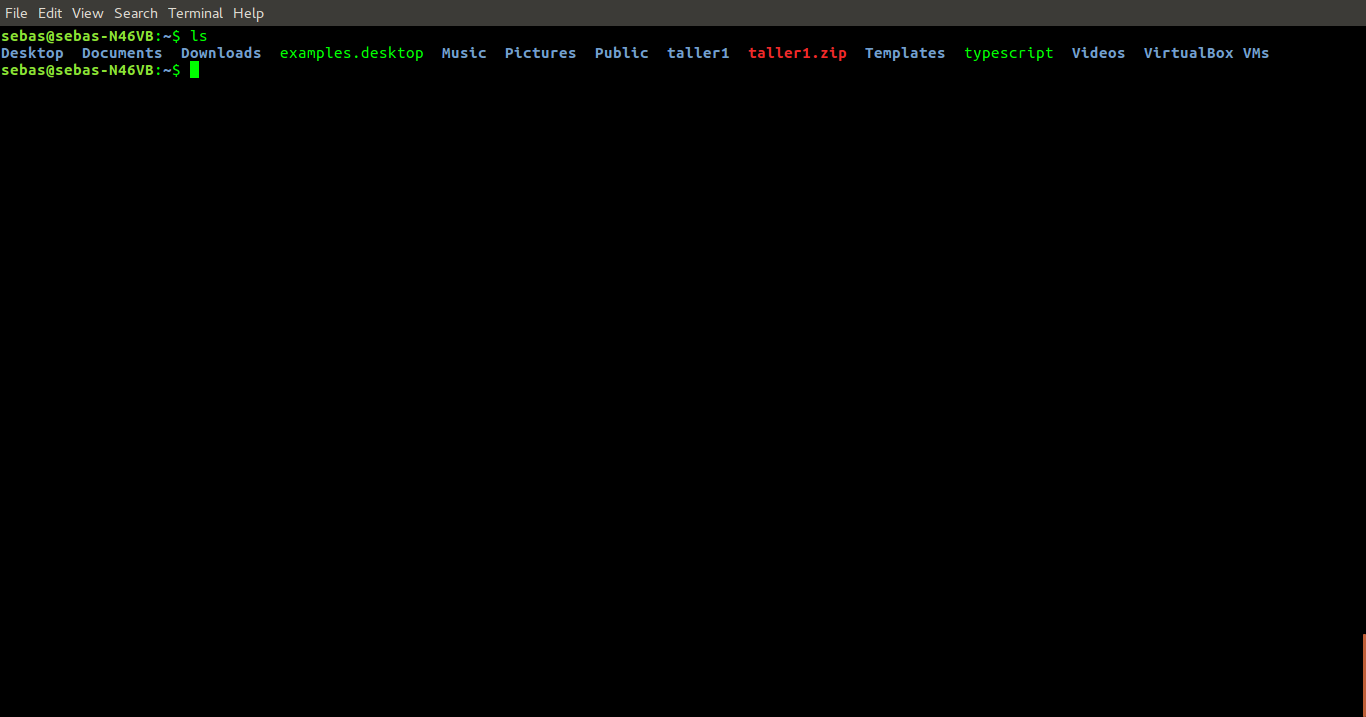
\includegraphics[width=\textwidth]{ls.png}
    \caption{Resultado de ejecutar ls.}
\end{figure}
Por defecto lista el contenido y lo organiza alfabéticamente. Este comportamiento puede cambiar cuando se agregan opciones, las opciones se usan para cambiar como se vera el contenido del directorio y se puede especificar el tipo de archivos que se desean visualizar.
\subsubsection{Opciones}
\begin{itemize}
	\item -a: Esta opción muestra todo, incluidos los archivos ocultos.\par
	    \begin{minipage}{\linewidth}
            \centering
            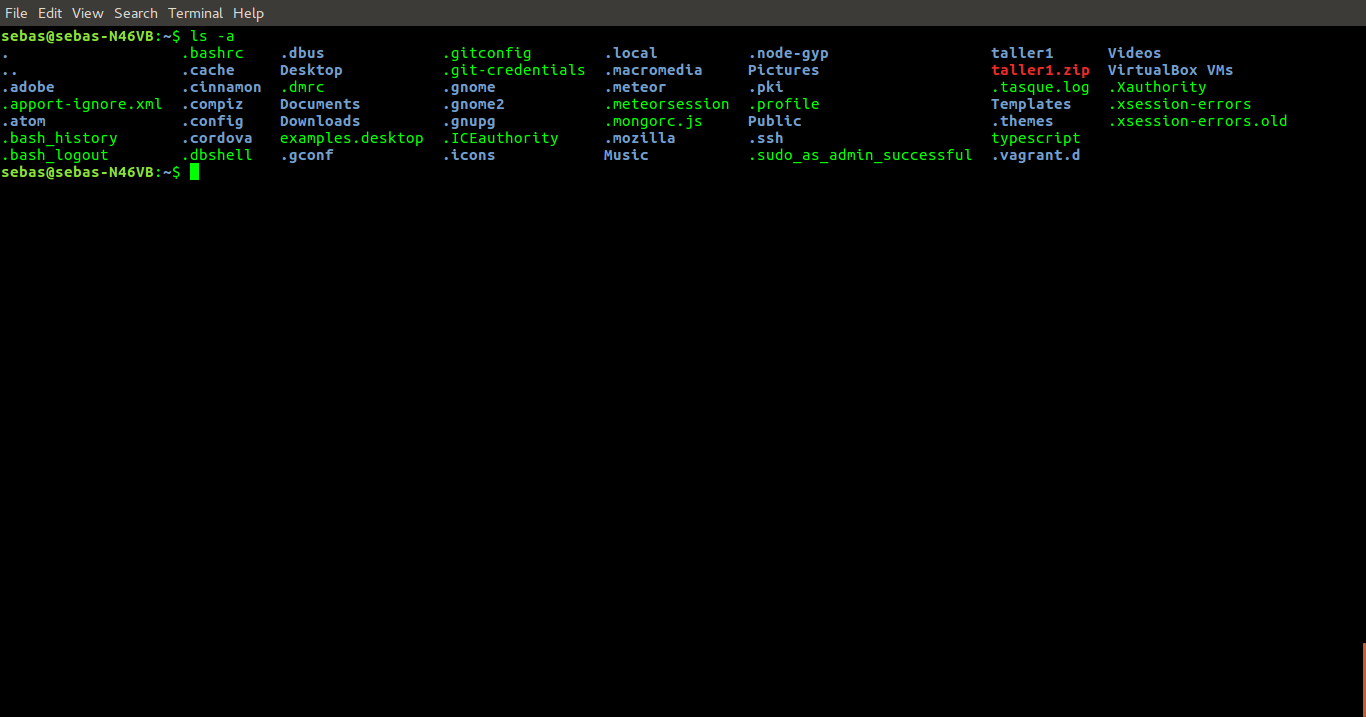
\includegraphics[width=\textwidth]{ls-a.png}
            \captionof{Ejecución ls -a.}
        \end{minipage}
    \item -l \emph{long listing format}: Lista el total de archivos en los directorios y subdirectorios, los nombres de los archivos en el directorio actual (sin mostrar los ocultos), los permisos de cada archivo y subdirectorio, el número de subdirectorios de cada directorio, el tamaño de cada archivo, la ultima fecha de modificación y el usuario que tiene permisos sobre el archivo o directorio.\par
	    \begin{minipage}{\linewidth}
            \centering
            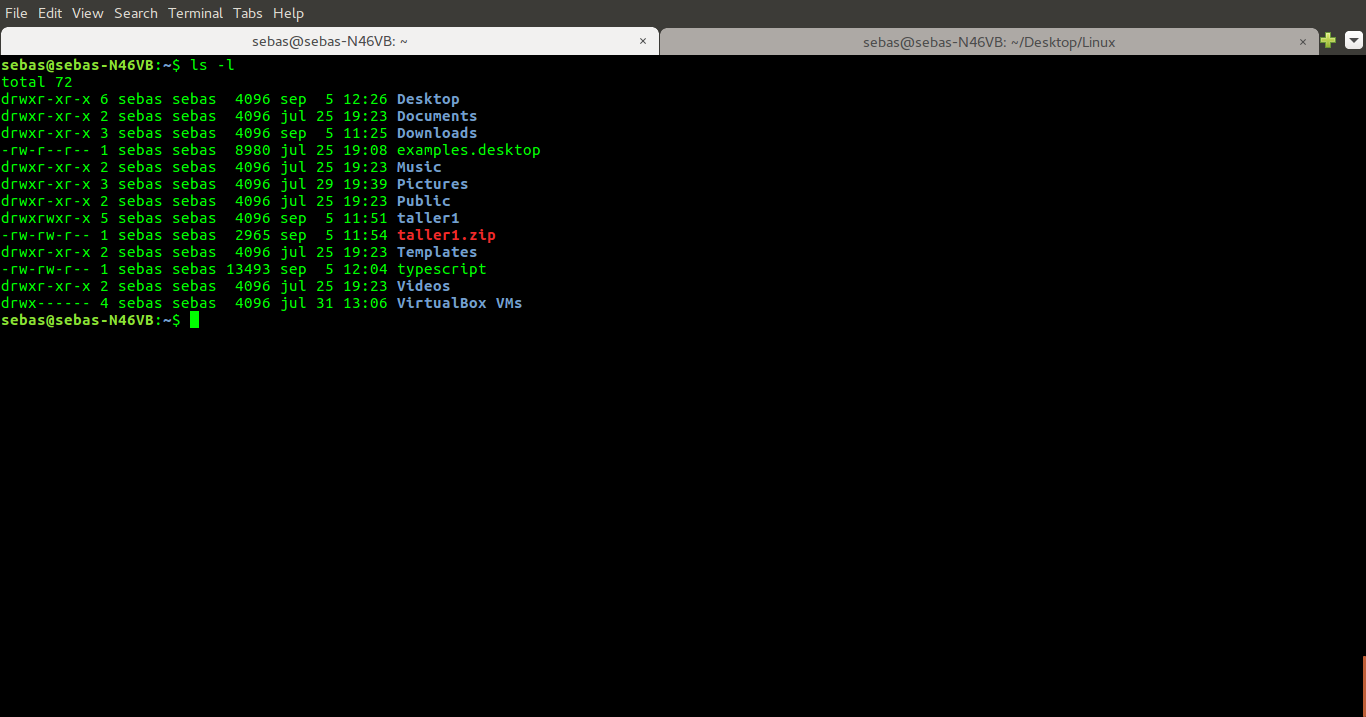
\includegraphics[width=\textwidth]{ls-l.png}
            \captionof{Ejecución ls -l.}
        \end{minipage}
    \item -laxo: Usa el mismo formato que \emph{-l}, la diferencia esta en que ésta opción si muestra los archivos y directorios ocultos.\par
    	\begin{minipage}{\linewidth}
            \centering
            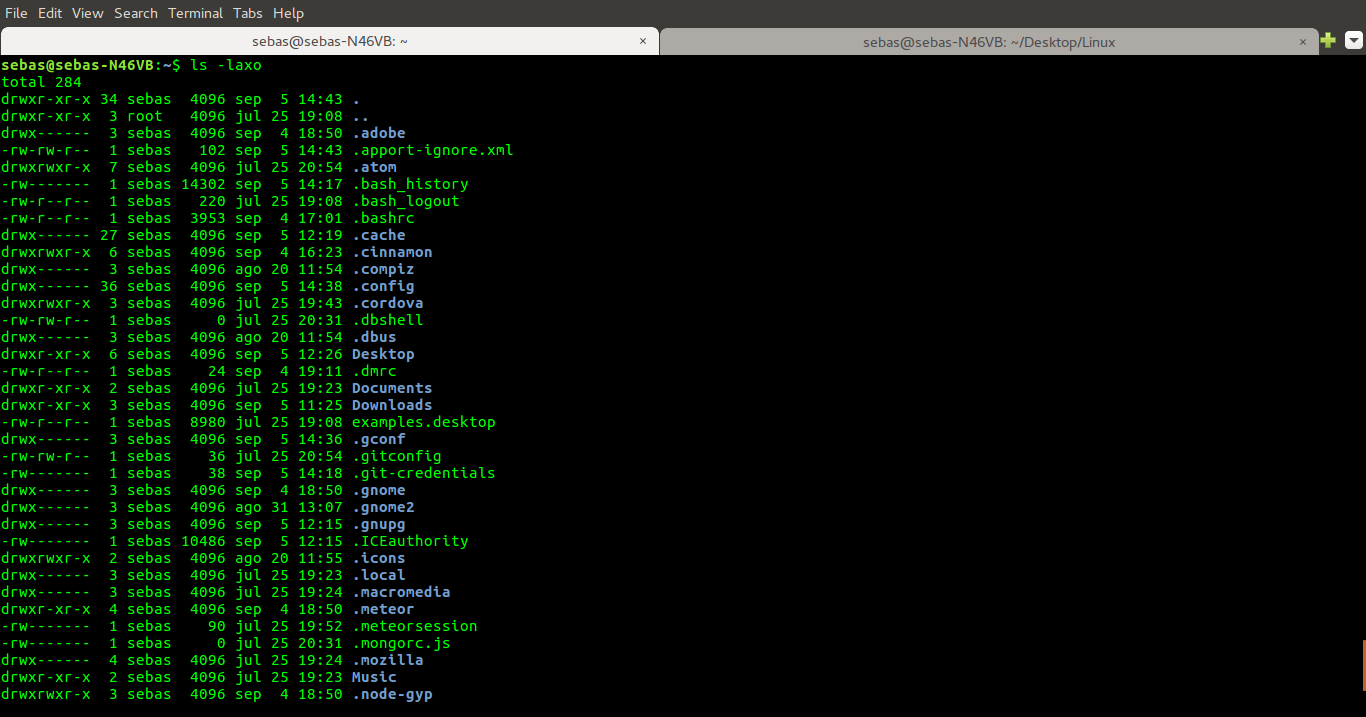
\includegraphics[width=\textwidth]{ls-laxo.png}
            \captionof{Ejecución ls -laxo.}
        \end{minipage}
    \item -d: Lista los subdirectorios del directorio en vez del contenido.\par
    	\begin{minipage}{\linewidth}
            \centering
            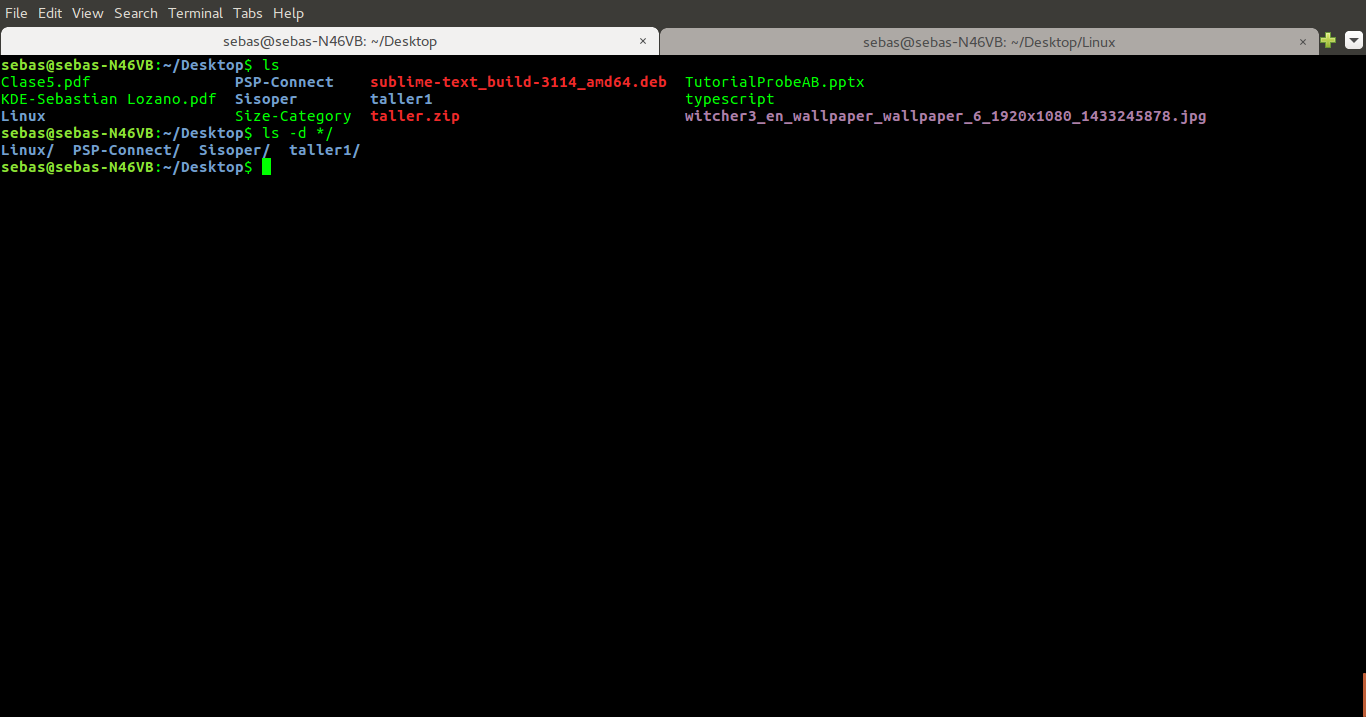
\includegraphics[width=\textwidth]{ls-d.png}
            \captionof{Ejecución ls -d del directorio actual.}
        \end{minipage}
\end{itemize}
\subsection{Comando \emph{grep} [opciones] patrón [archivo]}
Grep es el diminutivo de \emph{global regular expression print}, procesa el texto de un archivo línea por línea e imprime cuando encuentra una coincidencia. 
\begin{figure}[h]
    \centering
    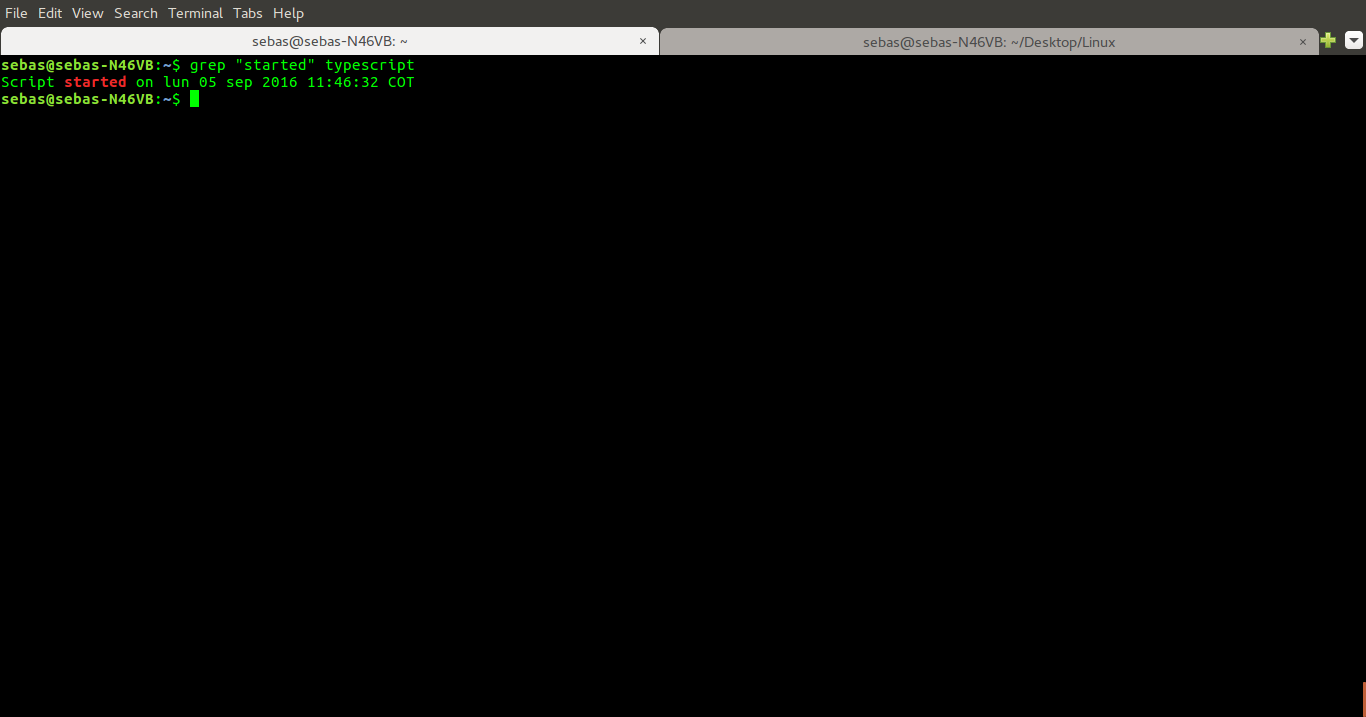
\includegraphics[width=\textwidth]{grep.png}
    \caption{Resultado de ejecutar grep buscando \emp{started} en typescript.}
\end{figure}
\subsubsection{Opciones}
\begin{itemize}
	\item -n: Muestra el número de la linea que arrojó coincidencia.\par
    	\begin{minipage}{\linewidth}
            \centering
            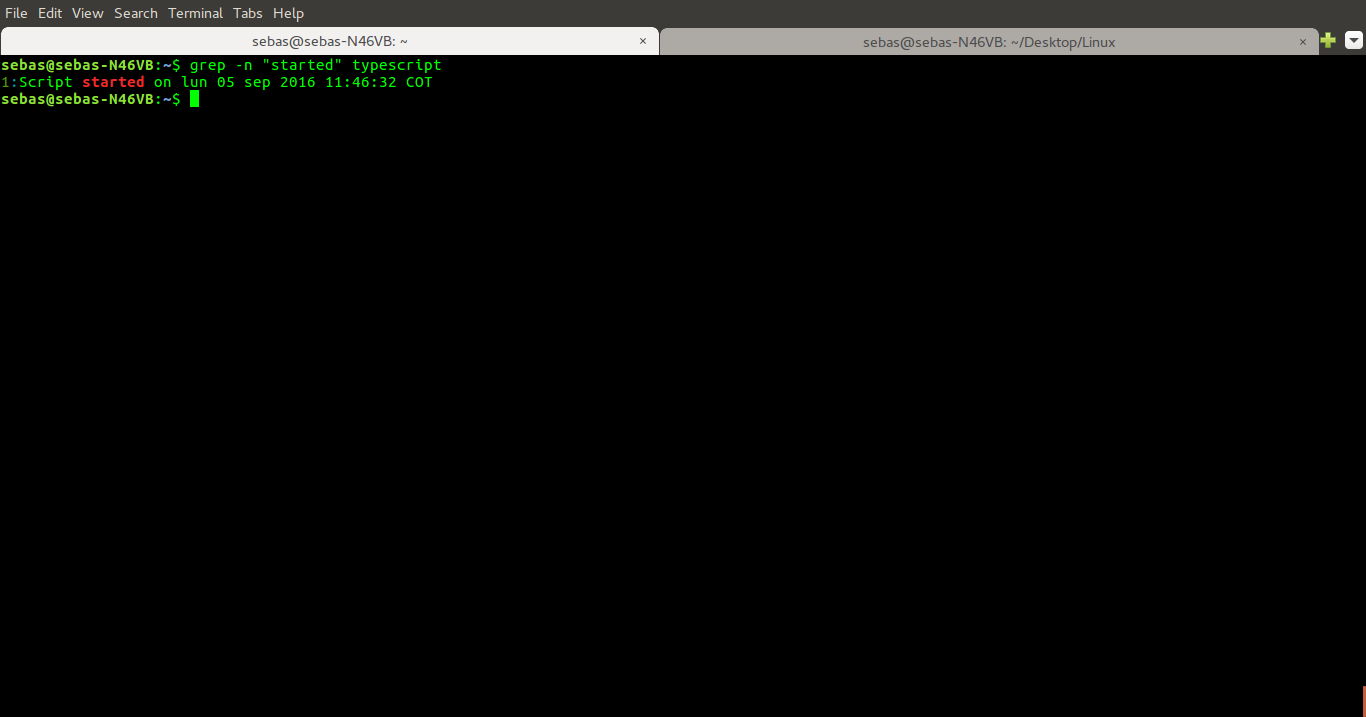
\includegraphics[width=\textwidth]{grep-n.png}
            \captionof{Ejecución grep -n.}
        \end{minipage}
    \item -n: La comparación ignora las mayúsculas y minúsculas.\par
    	\begin{minipage}{\linewidth}
            \centering
            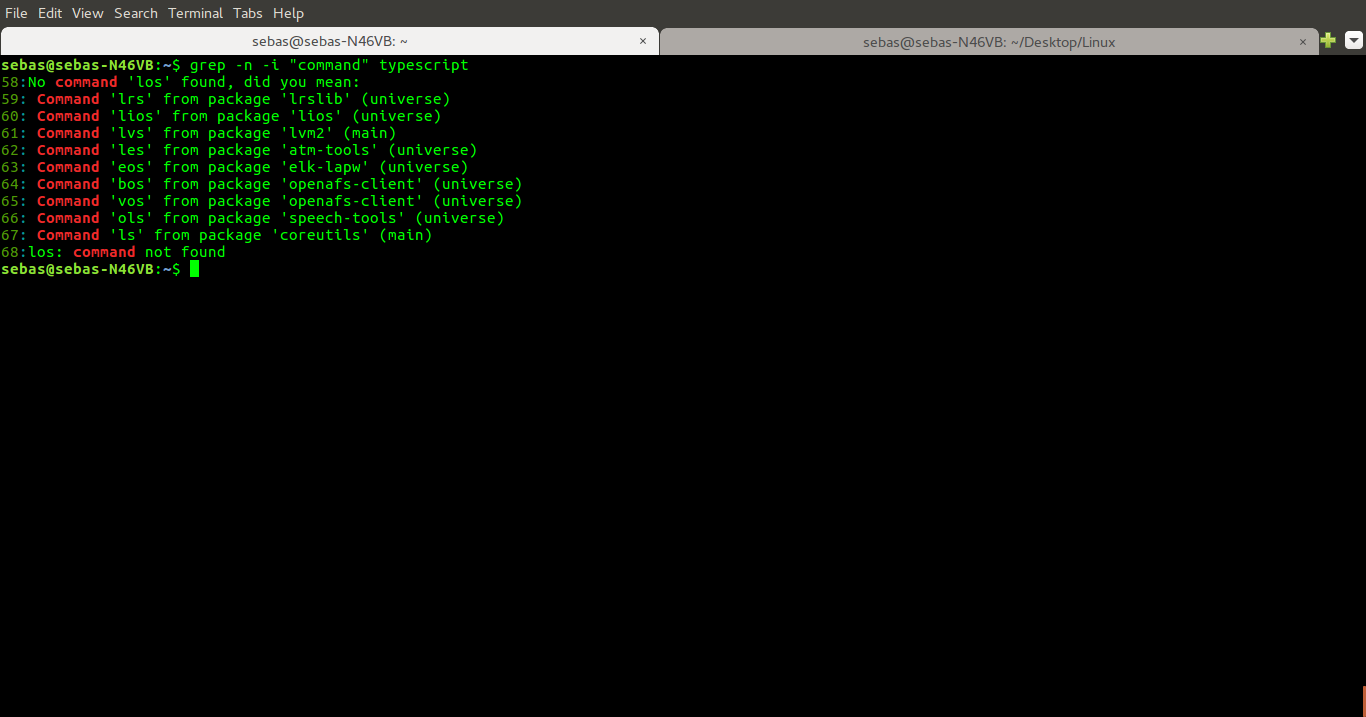
\includegraphics[width=\textwidth]{grep-i.png}
            \captionof{Ejecución grep -n.}
        \end{minipage}  
    \item -r: La comparación la realiza recursivamente dentro de cada subdirectorio, para este ejemplo se esta buscando en cualquier archivo.\par
        \begin{minipage}{\linewidth}
            \centering
            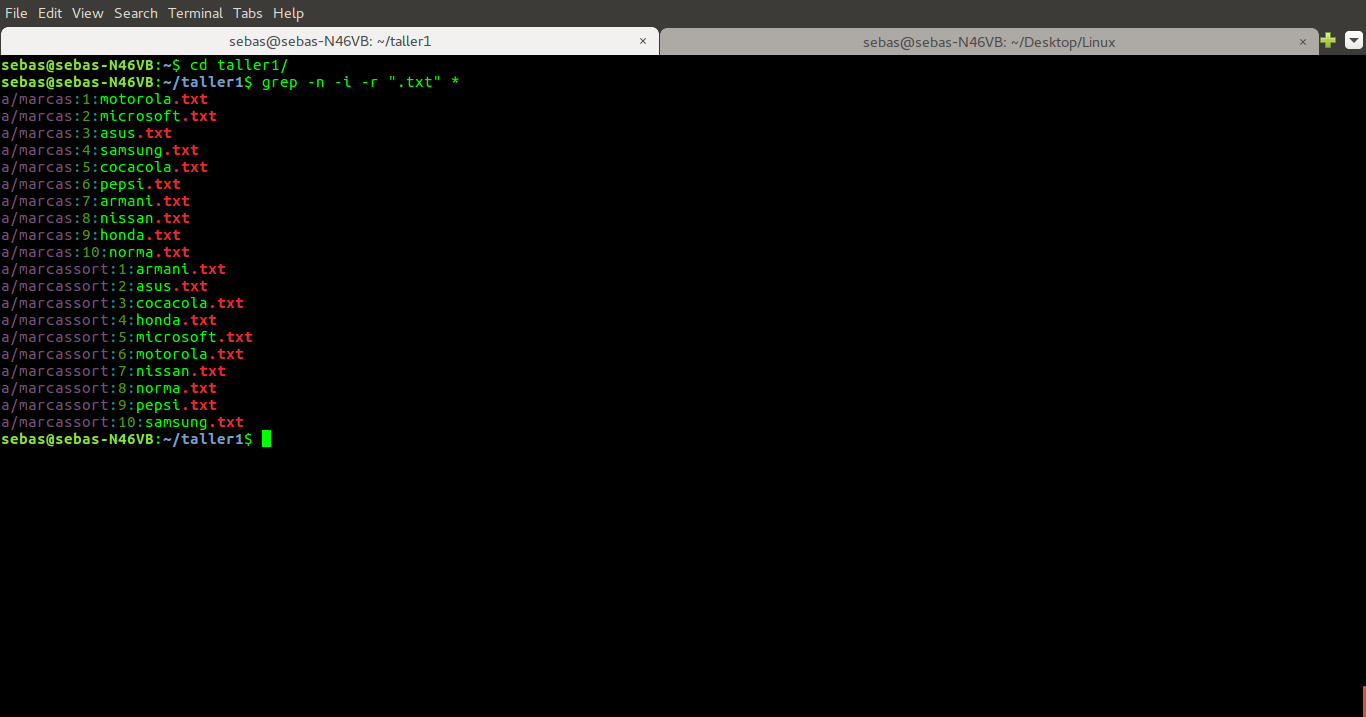
\includegraphics[width=\textwidth]{grep-r.png}
            \captionof{Ejecución grep -r.}
        \end{minipage}
\end{itemize}
\subsection{Comando \emph{sed} opciones [script] [archivo]}
Sed es el diminutivo de \emph{stream editor}, permite filtrar y reemplazar el texto de un archivo de entrada de acuerdo a las especificaciones del script. El script es obligatorio y puede ser especificado en la línea o puede encontrarse en un archivo.
\begin{figure}[h]
    \centering
    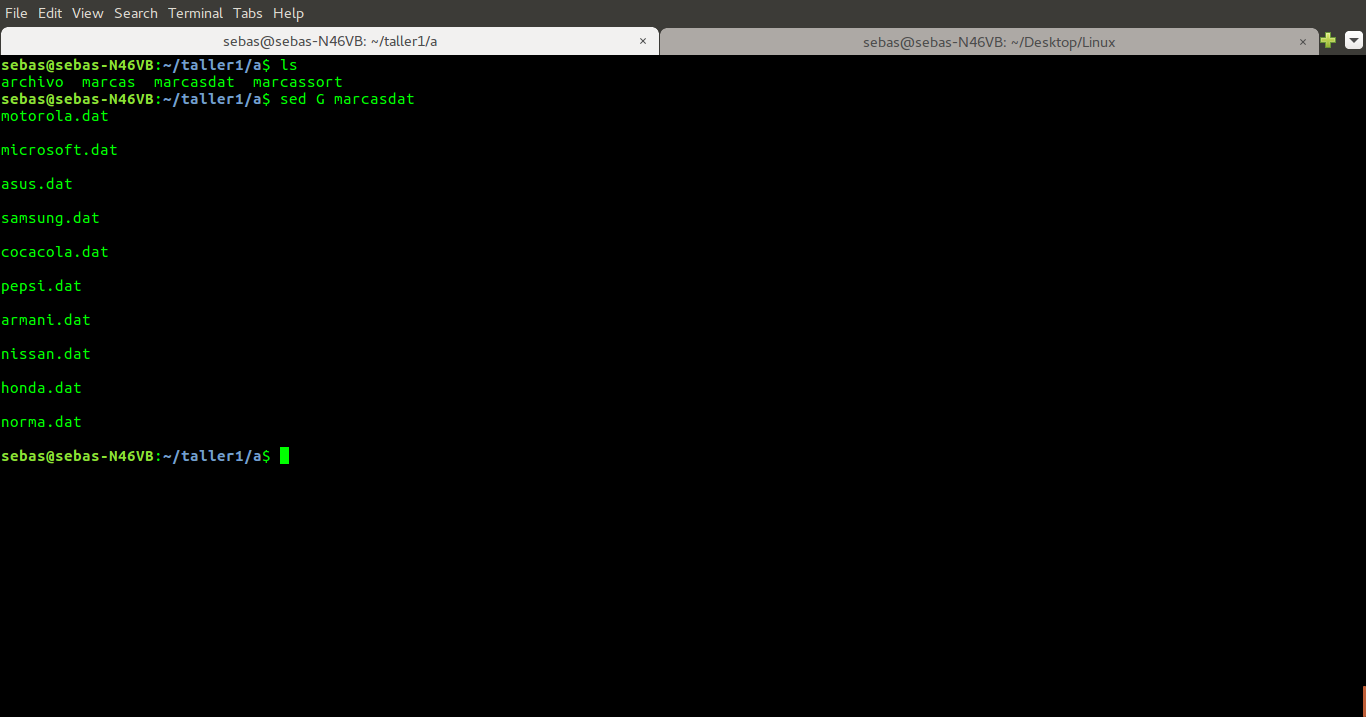
\includegraphics[width=\textwidth]{sed.png}
    \caption{Resultado de ejecutar sed con el comando G.}
\end{figure}
\subsubsection{Opciones}
\begin{itemize}
	\item -n: Elimina los prints automáticos.\par
        \begin{minipage}{\linewidth}
            \centering
            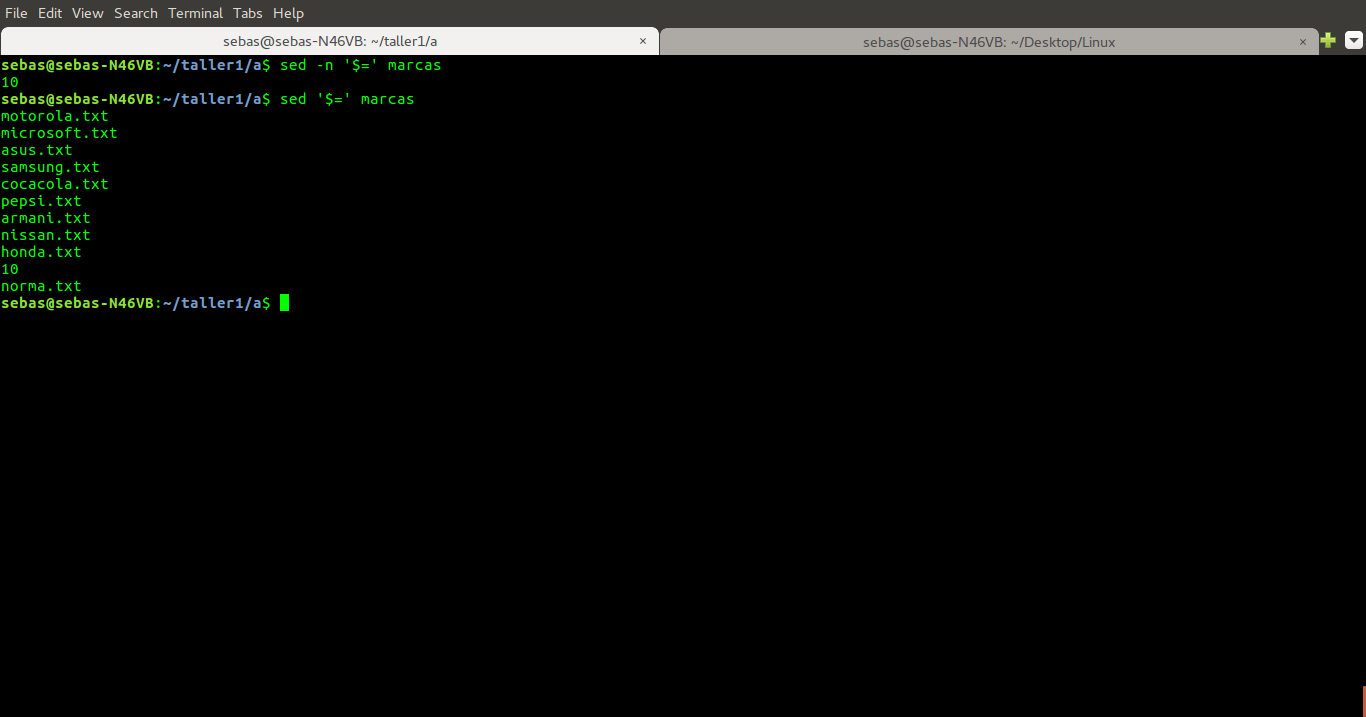
\includegraphics[width=\textwidth]{sed-n.png}
            \captionof{Ejecución sed -n.}
        \end{minipage}
\end{itemize}

\end{document}
